\usepackage[T1]{fontenc}
\usepackage{concrete}

\mode<all>
{
\setbeamerfont{block title}{size={}}
\usefonttheme{serif}
\usefonttheme{professionalfonts}
\setbeamercovered{invisible}
\useoutertheme[subsection=true3]{smoothbars}
\useinnertheme[shadow=true]{rounded}
\usecolortheme{orchid}
\usecolortheme{whale}
\setbeamertemplate{navigation symbols}{}
\setbeamertemplate{mini frames}[box]
\setbeamertemplate{itemize items}[triangle]
\setbeamertemplate{enumerate items}[square]

}

\usepackage[latin1]{inputenc}
\usepackage{xspace} % To get the right spacings in front of : and so on
\usepackage[english]{babel}
\usepackage{subfigure}
\usepackage{bussproofs}
\usepackage{pgf}
\usepackage{colortbl}
\usepackage{xcolor}
\usepackage{abbrevs}
\usepackage{coq}
\usepackage{cond}
\usepackage{tikz}

\def\PI{\name{PI}}
\def\shaded#1{{\color{black!50}#1}}
 
\EnableBpAbbreviations
\def\fCenter{\vdash}
\def\seq{\fCenter}

\hypersetup{
  pdftitle = Programing in Coq,
  pdfauthor = Matthieu Sozeau,
  pdfsubject = Theoretical Computer Science
 } 

\def\constr#1{\textsf{#1}}

\newcommand{\termgrammar}
{$\begin{array}{lcl}
    `a & \Coloneqq & x \\
    & | & \funml{}~x~:~`t "=>" `a \\
    & | & `a~`a \\ 
    & | & `a~`t \\
    & | & \text{\emph{constante}} \\
% & | & (`a,~`a) \\
    & | & (x \coloneqq `a,~`a~: `t) \\
    & | & \letml~x = `a ~\inml~`a \\
    & | & \letml~(x, y) = `a ~\inml~ `a

%    & | & \ifml~`a~\thenml~`a~\elseml~`a
  \end{array}$}

\newcommand{\typegrammarOrig}
{$\begin{array}{lcl}
    `t & \Coloneqq & x \\
    & | & `t "->" `t \\
    & | & `t~`t \\
    & | & \text{\emph{constante}} \\
    & | & `t * `t \\
    & | & \Sigma x : `t. `t \\
    & | & \lambda{}~x~:~s "=>" `t \\
    & | & `t~`a \\
    & | & \Pi x : `t. `t \\
    & | & \subset{x}{`t}{`t}
  \end{array}$}

\newcommand{\typegrammar}
{$\begin{array}{lcl}
    `t & \Coloneqq & x \\
    & | & `t~`t \\
    & | & `t~`a \\
    & | & \lambda{}~x~:~`t "=>" `t \\
    & | & \Pi x : `t. `t \\
    & | & \Sigma x : `t. `t \\
%    & | & `t * `t \\
    & | & \subset{x}{`t}{`t} \\
    & | & \Set \\
    & | & \Prop \\
    & | & \Type \\
    & | & \text{\emph{constante}} 
%    & & \\
%    \text{{\tt Inductive}} & \Coloneqq & ident
  \end{array}$}

\def\lang{en}
\newtheorem{theorem}{Th�or�me}[section]
\newtheorem{lemma}[theorem]{Lemme}
\newtheorem{fact}[theorem]{Fait}
\newtheorem{proposition}[theorem]{Proposition}
\newtheorem{definition}[theorem]{D�finition}
\newtheorem{example}[theorem]{Exemple}
\newtheorem{remark}[theorem]{Remarque}
\newtheorem{corrolary}[theorem]{Corrolaire}

\makeatletter

\newcommand{\UR}[2]{\RightLabel{\rulelabel{#1}}\UIC{#2}}
\newcommand{\URL}[2]{\LeftLabel{\rulelabel{#1}}\UIC{#2}}

\newboolean{displayLabels}
\setboolean{displayLabels}{true}

\newcommand{\LeftRuleLabel}[1]{
  \@ifnotmtarg{#1}
  {\ifthenelse{\boolean{displayLabels}}{\LeftLabel{\rulelabel{#1}}}{}}
}

\newcommand{\UAX}[4]{\AXC{#2}
  \LeftRuleLabel{#1}
  \@ifnotmtarg{#4}{\RightLabel{#4}}
  \UIC{#3}}

\newcommand{\BAX}[5]{\AXC{#2}\AXC{#3}
  \LeftRuleLabel{#1}
  \@ifnotmtarg{#5}{\RightLabel{#5}}
  \BIC{#4}}

\newcommand{\TAX}[6]{\AXC{#2}\AXC{#3}\AXC{#4}
  \LeftRuleLabel{#1}
  \@ifnotmtarg{#6}{\RightLabel{#6}}
  \TIC{#5}}

\newcommand{\QAX}[7]{\AXC{#2}\noLine\UIC{#3}\AXC{#4}\AXC{#5}
  \LeftRuleLabel{#1}
  \@ifnotmtarg{#7}{\RightLabel{#7}}
  \TIC{#6}}

\newcommand{\BR}[2]{\RightLabel{\rulelabel{#1}}\BIC{#2}}
\newcommand{\BRL}[2]{\LeftLabel{\rulelabel{#1}}\BIC{#2}}

\makeatother

%%% Local Variables: 
%%% mode: latex
%%% TeX-master: t
%%% End: 


\newcommand{\coqdocind}[1]{\textsf{#1}}
\newcommand{\coqdocconstr}[1]{\textsf{#1}}

\def\id{\coqdocid}
\def\ind{\coqdocind}
\def\constr{\coqdocconstr}
\def\kw{\coqdockw}
\def\class{\kw{class}~}
\def\tclass#1{\textsf{#1}}
\def\where{\kw{where}~}
\def\module#1{\texttt{#1}}

\title[Dependent Finger Trees in \Russell]{Programming Dependent Finger Trees with \Russell}

\author[Matthieu Sozeau]
{{\sc Matthieu Sozeau}}

\institute[]
{
  \LRI{}, Univ. Paris-Sud - \Demons{} Team \& \INRIAFuturs{} - \ProVal{} Project
}

\date
{\ProVal workgroup \\
April 2nd 2007}

\subject{Theoretical Computer Science}

\pgfdeclareimage[height=0.5cm]{ups-logo}{../figures/ups-logo}
\pgfdeclareimage[height=0.5cm]{lri-logo}{../figures/lri-logo}
\pgfdeclareimage[height=0.5cm]{inria-logo}{../figures/inria-logo}

\pgfdeclareimage[height=7.5cm]{depextr}{figures/bigpicextr}

\begin{document}

\begin{frame}[plain]
  \titlepage
  \vfill\hfill
  \pgfuseimage{ups-logo}
  ~
  \pgfuseimage{lri-logo}
  ~
  \pgfuseimage{inria-logo}
\end{frame}

\begin{frame}[plain]
  \frametitle{Flashback}
  \pgfuseimage{depextr}
\end{frame}

\frame{\tableofcontents}

\section{Original Finger Trees}

\subsection{An introduction}
\begin{frame}
  \frametitle{A quick tour of Finger Trees}
  
  \begin{itemize}
  \item A simple general purpose data structure (Hinze \& Paterson, 2006) ;
  \item Purely functional, nested datatype ;
  \item General purpose, parameterized data structure (gives sequences,
    priority queues, search trees...) ;
  \item Efficient deque operations (amortized constant time) and
    concatenation and splitting (logarithmic in smallest argument's
    size).
  \item Simple implementation compared to Kaplan \& Tarjan's
    catenable dequeues, efficient in practice.
  \end{itemize}
  
\end{frame}

\begin{frame}
  \frametitle{The Big Finger Tree Picture}
  \begin{center}
  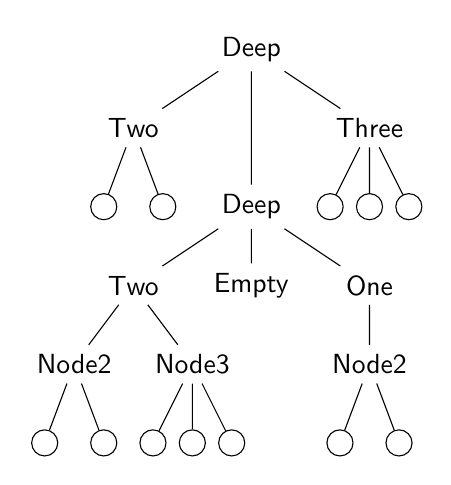
\begin{tikzpicture}
    \tikzstyle{every circle node}=[circle,draw]
    \node {\constr{Deep}}
    [level distance=1cm]
    child { node {\constr{Two}}
      [sibling distance=0.75cm]
      child { node[circle] { } }
      child { node[circle] {  } }
    }
    child[level distance=2cm] {
      node {\constr{Deep}}
      [level distance=1cm]
      child { node {\constr{Two}}
        child { node {\constr{Node2}}
          [sibling distance=0.75cm]
          child { node[circle] {} }
          child { node[circle] {} }}
        child { node {\constr{Node3}}
          [sibling distance=0.5cm]
          child { node[circle] {} }
          child { node[circle] {} }
          child { node[circle] {} }
        }
      }
      child { node {\constr{Empty}} }
      child { node {\constr{One}}
        child { node {\constr{Node2}}
          [sibling distance=0.75cm]
          child { node[circle] {} }
          child { node[circle] {} }
        }
      }
    }
    child { node {\constr{Three}}
      [sibling distance=0.5cm]
      child { node[circle] {} }
      child { node[circle] {} }
      child { node[circle] {} }
    };
  \end{tikzpicture} 
\end{center}  

\end{frame}

\subsection{In \Haskell}

\begin{frame}[t]
  \frametitle{A \emph{nested} datatype and its companions}
  \def\myv{\only<2->{\alert{\id{v} }}}
  \kw{data} \ind{FingerTree} \myv \id{a} = 
  \coqdoceol{}\coqdocindent{2.00em}| \constr{Empty} 
  \coqdoceol{}\coqdocindent{2.00em}| \constr{Single} \id{a}
  \coqdoceol{}\coqdocindent{2.00em}| \constr{Deep} \myv (\ind{Digit}
  \id{a}) (\ind{FingerTree} \myv (\ind{Node} \myv \id{a}))
  (\ind{Digit} \id{a})
  \medskip

  \kw{data} \ind{Node} \myv \id{a} = \constr{Node2} \myv \id{a}
  \id{a} | \constr{Node3} \myv \id{a} \id{a} \id{a}

  \medskip
  \kw{data} \ind{Digit} \id{a} = 
  \coqdoceol{}\coqdocindent{2.00em}| \constr{One} \id{a}
  \coqdoceol{}\coqdocindent{2.00em}| \constr{Two} \id{a} \id{a}
  \coqdoceol{}\coqdocindent{2.00em}| \constr{Three} \id{a} \id{a} \id{a}
  \coqdoceol{}\coqdocindent{2.00em}| \constr{Four} \id{a} \id{a} \id{a} \id{a}

\end{frame}

\begin{frame}
  \frametitle{A sample \ind{FingerTree}}
  \begin{center}
  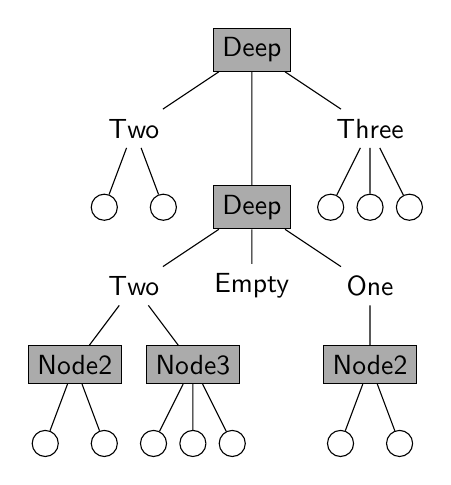
\begin{tikzpicture}
    \tikzstyle{every circle node}=[circle,draw]
    \node[draw,fill=black!33] {\constr{Deep}}
    [level distance=1cm]
    child { node {\constr{Two}}
      [sibling distance=0.75cm]
      child { node[circle] { } }
      child { node[circle] {  } }
    }
    child[level distance=2cm] {
      node[draw,fill=black!33] {\constr{Deep}}
      [level distance=1cm]
      child { node {\constr{Two}}
        child { node[draw,fill=black!33] {\constr{Node2}}
          [sibling distance=0.75cm]
          child { node[circle] {} }
          child { node[circle] {} }}
        child { node[draw,fill=black!33] {\constr{Node3}}
          [sibling distance=0.5cm]
          child { node[circle] {} }
          child { node[circle] {} }
          child { node[circle] {} }
        }
      }
      child { node {\constr{Empty}} }
      child { node {\constr{One}}
        child { node[draw,fill=black!33] {\constr{Node2}}
          [sibling distance=0.75cm]
          child { node[circle] {} }
          child { node[circle] {} }
        }
      }
    }
    child { node {\constr{Three}}
      [sibling distance=0.5cm]
      child { node[circle] {} }
      child { node[circle] {} }
      child { node[circle] {} }
    };
  \end{tikzpicture} 
  \end{center}
\end{frame}

\begin{frame}[t]
  \frametitle{Operating on a Finger Tree}
  
  \id{add\_left} :: \id{a} $"->"$ \ind{FingerTree} \id{v} \id{a} $"->"$
  \ind{FingerTree} \id{v} \id{a}\coqdoceol
  \id{add\_left} \id{a} \constr{Empty} = \constr{Single} \id{a}\coqdoceol
  \id{add\_left} \id{a} (\constr{Single} \id{b}) = \constr{Deep}
  (\constr{One} \id{a}) \constr{Empty} (\constr{One} \id{b})\coqdoceol
  \id{add\_left} \id{a} (\constr{Deep} \id{v} \id{pr} \id{m} \id{sf}) = $\ldots$
  \pause
  \begin{center}
  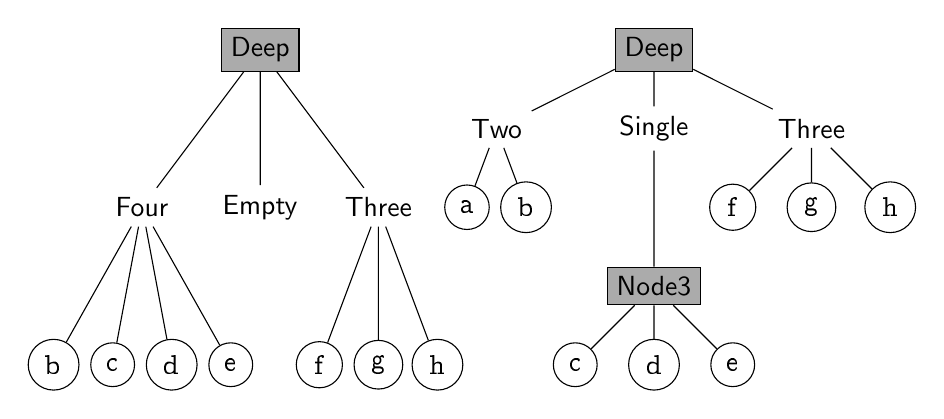
\begin{tikzpicture}
    \tikzstyle{every circle node}=[circle,draw]
    \node[draw,fill=black!33] {\constr{Deep}}
    [level distance=2cm,sibling distance=1.5cm]
    child { node {\constr{Four}}
      [sibling distance=0.75cm]
      child { node[circle] { b } }
      child { node[circle] { c } }
      child { node[circle] { d } }
      child { node[circle] { e } }
    }
    child { node {\constr{Empty}} }
    child { node {\constr{Three}}
      [sibling distance=0.75cm]
      child { node[circle] { f} }
      child { node[circle] { g } }
      child { node[circle] { h} }
    };
    \fill (5.0,.0) node[draw,fill=black!33] {\constr{Deep}}
    [level distance=1cm,sibling distance=2cm]
    child { node {\constr{Two}}
      [sibling distance=0.75cm]
      child { node[circle] { a } }
      child { node[circle] { b } }
    }
    child { 
      node {\constr{Single}}
      [level distance=2cm]
      child { node[draw,fill=black!33] {\constr{Node3}}
        [level distance=1cm,sibling distance=1cm]
        child { node[circle] { c } }
        child { node[circle] { d } }
        child { node[circle] { e } }
      }
    }
    child { node {\constr{Three}}
      [sibling distance=1cm]
      child { node[circle] { f } }
      child { node[circle] { g } }
      child { node[circle] { h } }
    };
  \end{tikzpicture}
\end{center}
\end{frame}

\begin{frame}
  \frametitle{A good set of primitive operations}
  
  \class \tclass{Monoid} \id{v} $"=>"$ \tclass{Measured} \id{v} \id{a} \where \coqdoceol
  \coqdocindent{1.00em}\id{measure} :: \id{a} $"->"$ \id{v}
  \medskip

  \id{add\_left},\id{add\_right},\coqdoceol
  
  \id{head}, \id{last} :: \tclass{Measured} \id{v} \id{a} $"=>"$ \ind{FingerTree} \id{v}
  \id{a} $"->"$ \id{a}\coqdoceol
  \id{tail}, \id{liat} :: \tclass{Measured} \id{v} \id{a} $"=>"$ \ind{FingerTree} \id{v}
  \id{a} $"->"$ \ind{FingerTree} \id{v} \id{a}
  \medskip
  \pause

  \id{app} :: \tclass{Measured} \id{v} \id{a} $"=>"$ \ind{FingerTree} \id{v}
  \id{a} $"->"$ \ind{FingerTree} \id{v} \id{a} $"->"$ 
  \coqdoceol\coqdocindent{1.00em}\ind{FingerTree} \id{v} \id{a}
  \medskip
  \pause

  \id{split} :: \tclass{Measured} \id{v} \id{a} $"=>"$ \ind{FingerTree} \id{v}
  \id{a} $"->"$ (\id{v} $"->"$ \ind{bool}) $"->"$ \id{v} $"->"$ \coqdoceol
  \coqdocindent{1.00em} \ind{Maybe} (\ind{FingerTree} \id{v} \id{a}) $*$
  \id{a} $*$ \ind{Maybe} (\ind{FingerTree} \id{v} \id{a})
  

  
\end{frame}


\section{Dependent Finger Trees}
\frame{\tableofcontents[currentsection]}

\subsection{Digits \& Nodes}
\begin{frame}[t]
  \frametitle{Digits}
\scriptsize{
  \coqdockw{Section} \coqdocid{Digit}.\coqdoceol
  \coqdocindent{1.00em}
  \coqdockw{Variable} \coqdocid{A} : \coqdockw{Type}.\coqdoceol
  \medskip
  
\coqdocindent{1.00em}
\coqdockw{Inductive} \coqdocid{digit} : \coqdockw{Type} := \coqdoceol
\coqdocindent{1.00em}
\coqor  \coqdocid{One} : \coqdocid{A} \ensuremath{\to} \coqdocid{digit}\coqdoceol
\coqdocindent{1.00em}
\coqor  \coqdocid{Two} : \coqdocid{A} \ensuremath{\to} \coqdocid{A} \ensuremath{\to} \coqdocid{digit}\coqdoceol
\coqdocindent{1.00em}
\coqor  \coqdocid{Three} : \coqdocid{A} \ensuremath{\to} \coqdocid{A} \ensuremath{\to} \coqdocid{A} \ensuremath{\to} \coqdocid{digit}\coqdoceol
\coqdocindent{1.00em}
\coqor  \coqdocid{Four} : \coqdocid{A} \ensuremath{\to} \coqdocid{A} \ensuremath{\to} \coqdocid{A} \ensuremath{\to} \coqdocid{A} \ensuremath{\to} \coqdocid{digit}.\coqdoceol

\medskip

\coqdocindent{1.00em}
\coqdockw{Definition} \coqdocid{full} \coqdocid{x} := \coqdockw{match} \coqdocid{x} \coqdockw{with} \coqdocid{Four} \coqdocid{\_} \coqdocid{\_} \coqdocid{\_} \coqdocid{\_} \ensuremath{\Rightarrow} \coqdocid{True} \coqor  \coqdocid{\_} \ensuremath{\Rightarrow} \coqdocid{False}  \coqdockw{end}.\coqdoceol
% \coqdocindent{1.00em}
% \coqdockw{Definition} \coqdocid{single} (\coqdocid{x} : \coqdocid{digit}) := \coqdockw{match} \coqdocid{x} \coqdockw{with} \coqdocid{One} \coqdocid{\_} \ensuremath{\Rightarrow} \coqdocid{True} \coqor  \coqdocid{\_} \ensuremath{\Rightarrow} \coqdocid{False} \coqdockw{end}.\coqdoceol
\pause

\medskip
\coqdocindent{1.00em}
\coqdockw{Program Definition} \coqdocid{add\_digit\_left} (\coqdocid{a} : \coqdocid{A}) (\coqdocid{d} : \coqdocid{digit} \coqor  \ensuremath{\lnot} \coqdocid{full} \coqdocid{d}) : \coqdocid{digit} :=\coqdoceol
\coqdocindent{2.00em}
\coqdockw{match} \coqdocid{d} \coqdockw{with}\coqdoceol
\coqdocindent{3.00em}
\coqor  \coqdocid{One} \coqdocid{x} \ensuremath{\Rightarrow} \coqdocid{Two} \coqdocid{a} \coqdocid{x}\coqdoceol
\coqdocindent{3.00em}
\coqor  \coqdocid{Two} \coqdocid{x} \coqdocid{y} \ensuremath{\Rightarrow} \coqdocid{Three} \coqdocid{a} \coqdocid{x} \coqdocid{y}\coqdoceol
\coqdocindent{3.00em}
\coqor  \coqdocid{Three} \coqdocid{x} \coqdocid{y} \coqdocid{z} \ensuremath{\Rightarrow} \coqdocid{Four} \coqdocid{a} \coqdocid{x} \coqdocid{y} \coqdocid{z}\coqdoceol
\coqdocindent{3.00em}
\coqor  \coqdocid{Four} \coqdocid{\_} \coqdocid{\_} \coqdocid{\_} \coqdocid{\_} \ensuremath{\Rightarrow} !\coqdoceol
\coqdocindent{2.00em}
\coqdockw{end}.\coqdoceol
\coqdocindent{1.00em}
\coqdockw{Next} \coqdockw{Obligation}.\coqdoceol
\noindent
\coqdocindent{2.00em}
\coqdocid{intros} ; \coqdocid{simpl} \coqdockw{in} \coqdocid{n} ; \coqdocid{auto}.\coqdoceol
\noindent
\coqdocindent{1.00em}
\coqdockw{Qed}.\coqdoceol

}


\end{frame}

\begin{frame}[t]
  \frametitle{Nodes}
\scriptsize{
\coqdocindent{1.00em}
\coqdockw{Variable} \coqdocid{v} : \coqdockw{Type}.\coqdoceol
\coqdocindent{1.00em}
\coqdockw{Variable} \coqdocid{mono} : \coqdocid{monoid} \coqdocid{v}.\coqdoceol
\medskip
\coqdocindent{1.00em}
\coqdockw{Notation} "'$\varepsilon$'" := \coqdocid{mempty} \coqdocid{mono}.\coqdoceol
\coqdocindent{1.00em}
\coqdockw{Infix} "$\cdot$" := \coqdocid{mappend} \coqdocid{mono} (\coqdocid{right} \coqdocid{associativity}, \coqdocid{at} \coqdocid{level} 20).\coqdoceol
\medskip
% \coqdocindent{1.00em}
% \coqdockw{Program Definition} \coqdocid{listMonoid} (\coqdocid{A} :
% \coqdockw{Type}) : \coqdocid{monoid} (\coqdocid{list} \coqdocid{A}) := \coqdoceol
% \coqdocindent{2.00em}
% \coqdocid{mkMonoid} \coqdocid{nil} \coqdocid{app} \coqdocid{\_} \coqdocid{\_} \coqdocid{\_}.\coqdoceol
% \medskip
\pause
\coqdocindent{1.00em}
\coqdockw{Section} \coqdocid{Nodes}.\coqdoceol
\coqdocindent{2.00em}
\coqdockw{Variable} \coqdocid{A} : \coqdockw{Type}.\coqdoceol
\coqdocindent{2.00em}
\coqdockw{Variable} \coqdocid{measure} : \coqdocid{A} \ensuremath{\to} \coqdocid{v}.\coqdoceol
\coqdocindent{2.00em}
\coqdockw{Notation} "'\ensuremath{\coqdoublebar}' \coqdocid{x} '\ensuremath{\coqdoublebar}'" $\coloneqq$ (\coqdocid{measure} \coqdocid{x}).\coqdoceol

\medskip
\coqdocindent{2.00em}
\coqdockw{Inductive} \coqdocid{node} : \coqdockw{Type} $\coloneqq$\coqdoceol
\coqdocindent{2.00em}
\coqor  \coqdocid{Node2} : \ensuremath{\forall} \coqdocid{x} \coqdocid{y}, \{ \coqdocid{s} : \coqdocid{v} \coqor  \coqdocid{s} = $\coqdoublebar$ \coqdocid{x} $\coqdoublebar$ $\cdot$ $\coqdoublebar$ \coqdocid{y} $\coqdoublebar$ \} \ensuremath{\to} \coqdocid{node}\coqdoceol
\coqdocindent{2.00em}
\coqor  \coqdocid{Node3} : \ensuremath{\forall} \coqdocid{x} \coqdocid{y} \coqdocid{z}, \{ \coqdocid{s} : \coqdocid{v} \coqor  \coqdocid{s} = $\coqdoublebar$ \coqdocid{x} $\coqdoublebar$ $\cdot$ $\coqdoublebar$ \coqdocid{y} $\coqdoublebar$ $\cdot$ $\coqdoublebar$ \coqdocid{z} $\coqdoublebar$ \} \ensuremath{\to} \coqdocid{node}.\coqdoceol
\pause
\medskip
\coqdocindent{2.00em}
\coqdockw{Program Definition} \coqdocid{node2} (\coqdocid{x} \coqdocid{y} : \coqdocid{A}) : \coqdocid{node} $\coloneqq$ \coqdoceol
\coqdocindent{3.00em}
\coqdocid{Node2} \coqdocid{x} \coqdocid{y} ($\coqdoublebar$ \coqdocid{x}
$\coqdoublebar$ $\cdot$ $\coqdoublebar$ \coqdocid{y}
$\coqdoublebar$).\coqdoceol
\medskip
\coqdocindent{2.00em}
\coqdockw{Program Definition} \coqdocid{node\_measure} (\coqdocid{n} : \coqdocid{node}) : \coqdocid{v} $\coloneqq$\coqdoceol
\coqdocindent{3.00em}
\coqdockw{match} \coqdocid{n} \coqdockw{with} \coqor  \coqdocid{Node2} \coqdocid{\_} \coqdocid{\_} \coqdocid{s} \ensuremath{\Rightarrow} \coqdocid{s} \coqor  \coqdocid{Node3} \coqdocid{\_} \coqdocid{\_} \coqdocid{\_} \coqdocid{s} \ensuremath{\Rightarrow} \coqdocid{s} \coqdockw{end}.\coqdoceol
}

\end{frame}

\subsection{A nested indexed datatype}
 
\begin{frame}[t]
  \frametitle{Dependent Finger Trees}
  \small{
  \coqdockw{Inductive} \coqdocid{fingertree} (\coqdocid{A} :
  \coqdockw{Type}) \only<2->{(\alert<2>{\coqdocid{measure} :
      \coqdocid{A} \ensuremath{\to} \coqdocid{v}})} : \only<3->{\alert{\coqdocid{v}} \ensuremath{\to} }\coqdockw{Type} $\coloneqq$\coqdoceol
  \coqor  \coqdocid{Empty} : \coqdocid{fingertree} \coqdocid{A}
  \only<2->{\alert<2>{\coqdocid{measure}}\only<3->{ \alert{$\varepsilon$}}}\coqdoceol
  \coqor  \coqdocid{Single} : \ensuremath{\forall} \coqdocid{x} :
  \coqdocid{A}, \coqdocid{fingertree} \coqdocid{A} \only<2->{\alert<2>{\coqdocid{measure}}\only<3->{ (\alert{\coqdocid{measure} \coqdocid{x}})}}\coqdoceol
  \coqor  \coqdocid{Deep} : \ensuremath{\forall} (\coqdocid{l} :
  \coqdocid{digit} \coqdocid{A})\only<3->{ (\alert{\coqdocid{m} : \coqdocid{v}})},\coqdoceol
  \coqdocindent{1.00em}
  \coqdocid{fingertree} (\alert<1>{\coqdocid{node} \coqdocid{A}}\only<2->{ \alert<2>{\coqdocid{measure}}})
  \only<2->{(\alert<2>{\coqdocid{node\_measure} \coqdocid{A}
      \coqdocid{measure}})\only<3->{\alert<3->{ \coqdocid{m}}}}
  \ensuremath{\to}\coqdoceol \coqdocindent{1.00em}
  \ensuremath{\forall} \coqdocid{r} : \coqdocid{digit} \coqdocid{A}, \coqdoceol
  \coqdocindent{1.00em}
  \coqdocid{fingertree} \coqdocid{A}\only<2->{
    \alert<2>{\coqdocid{measure}}\only<3->{\coqdoceol\coqdocindent{3.00em}(\alert{\coqdocid{digit\_measure} \coqdocid{measure} \coqdocid{l}
        $\cdot$ \coqdocid{m} $\cdot$ \coqdocid{digit\_measure}
        \coqdocid{measure} \coqdocid{r}})}}.
  \coqdoceol}

  \only<2>{
    \begin{center}
      \small{\coqdocid{node\_measure} \coqdocid{A}
      (\coqdocid{measure} : \coqdocid{A} \ensuremath{\rightarrow}
      \coqdocid{v})  : \coqdocid{node A measure}
      \ensuremath{\rightarrow} \coqdocid{v}}
    \end{center}
  }
  
\end{frame}

\begin{frame}[t]
  \frametitle{Adding to the left}

  \medskip
  \coqdockw{Program Fixpoint} \coqdocid{add\_left} \coqdocid{A}
  (\coqdocid{measure} : \coqdocid{A} \ensuremath{\to} \coqdocid{v})
  \coqdoceol
  \coqdocindent{1.00em}
  (\alert{\coqdocid{a}} : \coqdocid{A}) (\alert{\coqdocid{s}} : \coqdocid{v})
  (\coqdocid{t} : \coqdocid{fingertree} \coqdocid{measure} \coqdocid{s})
  \{\coqdocid{struct} \coqdocid{t}\} : \coqdoceol
  \coqdocindent{1.00em}
  \coqdocid{fingertree} \coqdocid{measure} (\alert{\coqdocid{measure} \coqdocid{a} $\cdot$ \coqdocid{s}}) $\coloneqq$\coqdoceol
  \coqdocindent{1.00em}
  \coqdockw{match} \coqdocid{t} \coqdockw{with}\coqdoceol
  \coqdocindent{2.00em}
  \coqor  \coqdocid{Empty} \ensuremath{\Rightarrow} \coqdocid{Single} \coqdocid{a}\coqdoceol
  \coqdocindent{2.00em}
  \coqor  \coqdocid{Single} \coqdocid{b} \ensuremath{\Rightarrow} \coqdocid{Deep} (\coqdocid{One} \coqdocid{a}) \coqdocid{Empty} (\coqdocid{One} \coqdocid{b})\coqdoceol
  \coqdocindent{2.00em}
  \coqor  \coqdocid{Deep} \coqdocid{pr} \coqdocid{st'} \coqdocid{t'} \coqdocid{sf} \ensuremath{\Rightarrow} \coqdoceol
  \coqdocindent{3.00em}
  \only<1>{$\cdots$}\only<2->{
  \coqdockw{match} \coqdocid{pr} \coqdockw{with}\coqdoceol
  \coqdocindent{4.00em}
  \coqor  \coqdocid{Four} \coqdocid{b} \coqdocid{c} \coqdocid{d}
  \coqdocid{e} \ensuremath{\Rightarrow}\coqdoceol
  \coqdocindent{5.00em}
  \coqdockw{let} \coqdocid{sub} $\coloneqq$ \coqdocid{add\_left} (\alert{\coqdocid{node3} \coqdocid{measure} \coqdocid{c} \coqdocid{d} \coqdocid{e}}) \coqdocid{t'} \coqdockw{in}\coqdoceol
  \coqdocindent{6.00em}
  \coqdocid{Deep} (\coqdocid{Two} \coqdocid{a} \coqdocid{b}) \coqdocid{sub} \coqdocid{sf}\coqdoceol
  \coqdocindent{4.00em}
  \coqor  \coqdocid{x} \ensuremath{\Rightarrow} \coqdocid{Deep} (\alert{\coqdocid{add\_digit\_left} \coqdocid{a} \coqdocid{pr}}) \coqdocid{t'} \coqdocid{sf}\coqdoceol
  \coqdocindent{3.00em}
  \coqdockw{end}}\coqdoceol
  \coqdocindent{1.00em}
  \coqdockw{end}.\coqdoceol
  
\end{frame}

\begin{frame}
  \frametitle{Concatenation}

  \begin{block}{Two hundred lines, one hundred obligations concatenation}
    \coqdocindent{1.00em}
    \coqdockw{Definition} \coqdocid{app} (\coqdocid{A} : \coqdockw{Type}) (\coqdocid{measure} : \coqdocid{A} \ensuremath{\to} \coqdocid{v}) \coqdoceol
    \coqdocindent{2.00em}
    (\coqdocid{xs} : \coqdocid{v}) (\coqdocid{x} : \coqdocid{fingertree} \coqdocid{measure} \coqdocid{xs})\coqdoceol
    \coqdocindent{2.00em}
    (\coqdocid{ys} : \coqdocid{v}) (\coqdocid{y} : \coqdocid{fingertree} \coqdocid{measure} \coqdocid{ys}) : \coqdoceol
    \coqdocindent{2.00em}
    \coqdocid{fingertree} \coqdocid{measure} (\coqdocid{xs} $\cdot$
    \coqdocid{ys}).\coqdoceol
  \end{block}
  
\end{frame}

\begin{frame}
  \frametitle{Splitting nodes}
  
  \small{\coqdocindent{1.00em}
\coqdockw{Program Definition} \coqdocid{splitNode} (\coqdocid{p} : \coqdocid{v} \ensuremath{\to} \coqdocid{bool}) (\coqdocid{i} : \coqdocid{v}) (\coqdocid{n} : \coqdocid{node} \coqdocid{measure}) : \coqdoceol
\coqdocindent{1.00em}
\{ \coqdocid{s} : \coqdocid{split} \shaded{(\coqdockw{fun} \coqdocid{A} \ensuremath{\Rightarrow} \coqdocid{option} (\coqdocid{digit} \coqdocid{A}))} \coqdocid{A} \coqor  \coqdockw{let} (\coqdocid{l}, \coqdocid{x}, \coqdocid{r}) $\coloneqq$ \coqdocid{s} \coqdockw{in}\coqdoceol
\coqdocindent{2.00em}
\coqdockw{let} \coqdocid{ls} $\coloneqq$ \shaded{\coqdocid{option\_digit\_measure} \coqdocid{measure} \coqdocid{l}} \coqdockw{in}\coqdoceol
\coqdocindent{2.00em}
\coqdockw{let} \coqdocid{rs} $\coloneqq$ \shaded{\coqdocid{option\_digit\_measure} \coqdocid{measure} \coqdocid{r}} \coqdockw{in}\coqdoceol
\coqdocindent{2.00em}
\coqdocid{node\_measure} \coqdocid{n} = \coqdocid{ls} $\cdot$ $\coqdoublebar$ \coqdocid{x} $\coqdoublebar$ $\cdot$ \coqdocid{rs} \ensuremath{\land}\coqdoceol
\coqdocindent{2.00em}
(\coqdocid{l} = \coqdocid{None} \ensuremath{\lor} \coqdocid{p} (\coqdocid{i} $\cdot$ \coqdocid{ls}) = \coqdocid{false}) \ensuremath{\land}\coqdoceol
\coqdocindent{2.00em}
(\coqdocid{r} = \coqdocid{None} \ensuremath{\lor} \coqdocid{p}
(\coqdocid{i} $\cdot$ \coqdocid{ls} $\cdot$ $\coqdoublebar$ \coqdocid{x}
$\coqdoublebar$) = \coqdocid{true})\} $\coloneqq$ $\ldots$}
\end{frame}

\frame{\tableofcontents[currentsection]}

\subsection{Instantiation: random-access sequences}

\begin{frame}
  \frametitle{A ``simple'' version}
  
  \coqdockw{Program Definition} \coqdocid{sizeMonoid} := \coqdoceol
  \coqdocindent{1.00em}@\coqdocid{mkMonoid} \coqdocind{nat} \constr{0} \coqdocid{plus} \coqdocid{\_} \coqdocid{\_} \coqdocid{\_}.\coqdoceol
  \pause
  \medskip
  \coqdockw{Program Definition} \coqdocid{measure} (\coqdocid{x} :
  \coqdocid{A}) : \coqdocid{v} := 1.
  \coqdoceol
  \medskip
  \coqdockw{Definition} \coqdocid{seq} := \coqdoceol\coqdocindent{1.00em}
  \{ \coqdocid{n} : \coqdocind{nat} \& \coqdocind{fingertree}
  \coqdocid{sizeMonoid} \coqdocid{measure} \coqdocid{n} \}.
  \coqdoceol
  \pause

  \medskip
  \coqdockw{Definition} \coqdocid{length} (\coqdocid{x} :
  \coqdocid{seq}) := 
  \coqdockw{let} (\coqdocid{s}, \coqdocid{seq}) := \coqdocid{x} \coqdockw{in} \coqdocid{s}.\coqdoceol
  \medskip
  \pause

  \coqdockw{Program Definition} \coqdocid{nth} \coqdocid{x} (\coqdocid{i} : \coqdocind{nat} \coqor  \coqdocid{i} < \coqdocid{length} \coqdocid{x}) : \coqdocid{A} := \coqdoceol
  \coqdocindent{1.00em}
  \coqdockw{dest} \coqdocid{x} \coqdockw{as} \coqdocid{existT} \coqdocid{s} \coqdocid{t} \coqdockw{in}\coqdoceol
  \coqdocindent{1.00em}
  \coqdockw{dest} \coqdocid{split\_tree} (\coqdocid{lt} \coqdocid{i}) 0 \coqdocid{t} \coqdockw{as} \coqdocconstr{mkTreeSplit} \coqdocid{\_} \coqdocid{\_} \coqdocid{x} \coqdocid{\_} \coqdocid{\_} \coqdockw{in} \coqdocid{x}.\coqdoceol
  \medskip
  \alert{Relies on invariants of the Monoid and measure}.

\end{frame}

\begin{frame}
  \frametitle{A dependent version: the measure gives the semantics}

  \coqdockw{Definition} \coqdocid{below} \coqdocid{i} := \{ \coqdocid{x} : \coqdocid{nat} | \coqdocid{x} $<$ \coqdocid{i} \}.\coqdoceol
  \medskip
  \coqdockw{Definition} \coqdocid{v} := \{ \coqdocid{i} : \coqdocid{nat} \& (\coqdocid{below} \coqdocid{i} \ensuremath{\to} \coqdocid{A}) \}.\coqdoceol
  \medskip
  \pause
  \coqdockw{Program Definition} $\varepsilon$ : \coqdocid{v} := 0 $\Yleft$ (\coqdockw{fun} \coqdocid{\_} \ensuremath{\Rightarrow} !).\coqdoceol
  \coqdockw{Program Definition} \coqdocid{append} (\coqdocid{xs} \coqdocid{ys} : \coqdocid{v}) : \coqdocid{v} := \coqdoceol
  \coqdocindent{1.00em}
  \coqdockw{let} (\coqdocid{n}, \coqdocid{fx}) := \coqdocid{xs} \coqdockw{in}
  \coqdockw{let} (\coqdocid{m}, \coqdocid{fy}) := \coqdocid{ys} \coqdockw{in}\coqdoceol
  \coqdocindent{2.00em}
  (\coqdocid{n} + \coqdocid{m}) $\Yleft$ \coqdoceol
  \coqdocindent{3.00em}
  (\coqdockw{fun} \coqdocid{i} \ensuremath{\Rightarrow} \coqdockw{if}
  \coqdocid{lt\_ge\_dec} \coqdocid{i} \coqdocid{n} \coqdockw{then}
  \coqdocid{fx} \coqdocid{i} \coqdockw{else} \coqdocid{fy}
  (\coqdocid{i} - \coqdocid{n})).\coqdoceol
  \medskip
  \coqdockw{Program Definition} \coqdocid{seqMonoid} : \id{monoid}
  \id{v} := \coqdoceol\coqdocindent{1.00em}
  @\coqdocid{mkMonoid} \coqdocid{v} $\varepsilon$ \coqdocid{append} \coqdocid{\_} \coqdocid{\_} \coqdocid{\_}.\coqdoceol
  \pause
  \medskip
  \coqdockw{Program Definition} \coqdocid{measure} (\coqdocid{x} : \coqdocid{A}) : \coqdocid{v} := 1 $\Yleft$ (\coqdockw{fun} \coqdocid{\_} \ensuremath{\Rightarrow} \coqdocid{x}).\coqdoceol  
  
\end{frame}

\begin{frame}
  \frametitle{The sequence and its operations}
    
  \coqdockw{Definition} \coqdocid{seq} (\coqdocid{x} : \coqdocid{v}) := \coqdocid{fingertree} \coqdocid{seqMonoid} \coqdocid{measure} \coqdocid{x}.\coqdoceol
  \medskip
  \coqdockw{Program Fixpoint} \coqdocid{make} (\coqdocid{i} :
  \coqdocind{nat}) (\coqdocid{v} : \coqdocid{A}) \{ \coqdocid{struct}
  \coqdocid{i} \} : \coqdoceol \coqdocindent{1.00em} \coqdocid{seq} (\coqdocid{i} $\Yleft$ (\coqdockw{fun} \coqdocid{\_} \ensuremath{\Rightarrow} \coqdocid{v})). \coqdoceol
  \medskip
  \pause
  \coqdockw{Program Definition} \coqdocid{get} (\coqdocid{i} : \coqdocind{nat}) (\coqdocid{m} : \coqdocid{below} \coqdocid{i} \ensuremath{\to} \coqdocid{A}) \coqdoceol
  \coqdocindent{1.00em}
  (\coqdocid{x} : \coqdocid{seq} (\coqdocid{i} $\Yleft$ \coqdocid{m})) (\coqdocid{j} : \coqdocid{below} \coqdocid{i}) : \{ \coqdocid{value} : \coqdocid{A} | \coqdocid{m} \coqdocid{j} = \coqdocid{value} \}.\coqdoceol
  \medskip
  \pause
  \coqdockw{Program Definition} \coqdocid{set} (\coqdocid{i} : \coqdocind{nat}) (\coqdocid{m} : \coqdocid{below} \coqdocid{i} \ensuremath{\to} \coqdocid{A})  \coqdoceol
  \coqdocindent{1.00em}
  (\coqdocid{x} : \coqdocid{seq} (\coqdocid{i} $\Yleft$ \coqdocid{m})) (\coqdocid{j} : \coqdocid{below} \coqdocid{i}) (\coqdocid{value} : \coqdocid{A}) \coqdoceol
  \coqdocindent{1.00em}
  :  \coqdocid{seq} (\coqdocid{i} $\Yleft$ (\coqdockw{fun} \coqdocid{idx} : \coqdocid{below} \coqdocid{i} \ensuremath{\Rightarrow} \coqdockw{if} \coqdocid{eq\_nat\_dec} \coqdocid{idx} \coqdocid{j} \coqdockw{then} \coqdocid{value} \coqdockw{else} \coqdocid{m} \coqdocid{idx})).\coqdoceol
  
\end{frame}

\begin{frame}
  \frametitle{Theorems for free!}


  \medskip
  \coqdockw{Program Lemma} \coqdocid{get\_set} \coqdocid{i} \coqdocid{m} (\coqdocid{x} : \coqdocid{seq} (\coqdocid{i} $\Yleft$ \coqdocid{m})) (\coqdocid{j} : \coqdocid{below} \coqdocid{i}) \coqdoceol
  \coqdocindent{1.00em}
  (\coqdocid{value} : \coqdocid{A}) : \coqdocid{value} = \coqdocid{get} (\coqdocid{set} \coqdocid{x} \coqdocid{j} \coqdocid{value}) \coqdocid{j}.\coqdoceol
  \medskip

  \medskip
  \coqdockw{Program Lemma} \coqdocid{get\_set\_diff} \coqdocid{i} \coqdocid{m} (\coqdocid{x} : \coqdocid{seq} (\coqdocid{i} $\Yleft$ \coqdocid{m})) \coqdoceol
  \coqdocindent{1.00em}
  (\coqdocid{j} : \coqdocid{below} \coqdocid{i}) (\coqdocid{value} : \coqdocid{A}) (\coqdocid{k} : \coqdocid{below} \coqdocid{i}) : \coqdoceol
  \coqdocindent{1.00em}
  \coqdocid{j} \ensuremath{\not=} \coqdocid{k} \ensuremath{\rightarrow}
  \coqdocid{get} \coqdocid{x} \coqdocid{k} = \coqdocid{get}
  (\coqdocid{set} \coqdocid{x} \coqdocid{j} \coqdocid{value})
  \coqdocid{k}.\coqdoceol
  \medskip


\end{frame}

\section*{Conclusion}
\begin{frame}
  \frametitle{Finger Trees with \Russell}
  
  \begin{block}{The development}
    \begin{itemize}
    \item Certified implementation of Finger Trees. 
      Certified implementation of sequences built on top of Finger Trees.
    \item $\sim$ 1200 lines of specification, $\sim$ 1400 of proof, mostly unchanged
      code.
    \item Extracts to \Haskell and \Ocaml (with magic).
    \end{itemize}
  \end{block}
  \pause
  \begin{block}{Conclusions}
    \begin{itemize}
    \item[+] \Program scales ;
    \item[+] Subset types arise naturally ;
    \item[+] Dependent types are a powerful specification tool ;      
    \item[--] Need more language technology, e.g: overloading ;
    \item[--] Some difficulties with reasoning and computing.
    \end{itemize}   
  \end{block}
  
\end{frame}

\begin{frame}
  \frametitle{The End}
  \centering{
    \begin{center}
      \url{http://www.lri.fr/~sozeau/research/russell/fingertrees.en.html}
    \end{center} 
  }
\end{frame}

\end{document}

%%% Local Variables: 
%%% mode: latex
%%% TeX-master: "slides"
%%% LaTeX-command: "x=pdf; TEXINPUTS=\"~/research/publication/styles:..:../style:../figures:\" ${pdfx}latex"
%%% TeX-PDF-mode: t
%%% TeX-view-style: (("." "~/bin/openpdf %s.pdf"))
%%% End: 
